% !TEX root = main.tex
\section{アクチュエータ,センサの動作確認}

\subsection{2軸ロボット実験装置におけるアクチュエータとセンサ}

\begin{figure}[H]
    \centering
    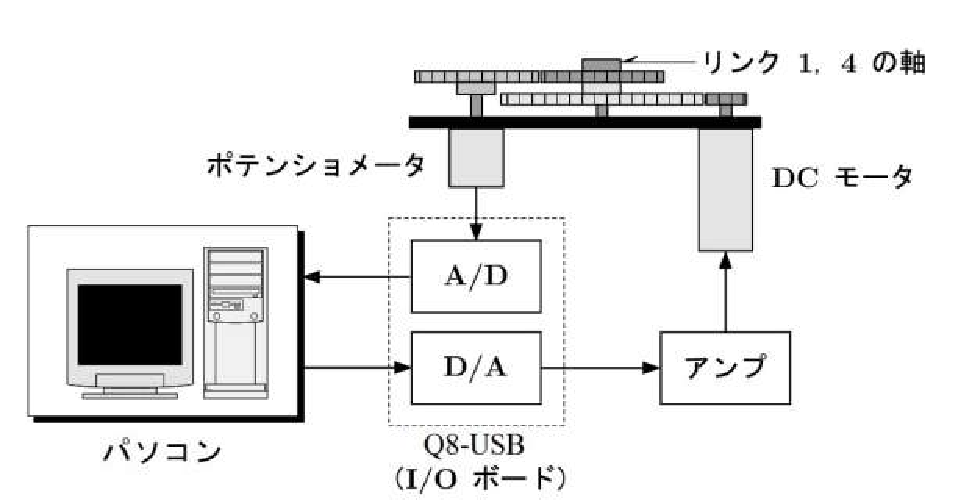
\includegraphics[width=0.8\linewidth]{figure/actuator_sensor.pdf}
    \caption{アクチュエータ(DCモータ)とセンサ(ポテンショメータ)}
    \label{fig:actuator_sensor}
\end{figure}

図\ref{fig:actuator_sensor}に示すように,2軸ロボット実験装置はリンク1,リンク4がギアを介してDCモータにより回転するようになっている.
DCモータを駆動させるためにパソコンにより計算された指令電圧は,I/OボードQ8-USBでD/A変換された後,アンプを介してDCモータに入力される.
また,リンク1,リンク4の回転角は角度センサであるポテンショメータにより電圧値として検出され,I/OボードQ8-USBでA/D変換された後,パソコンに取り込まれている.
